\documentclass{article}
\author{Max Springenberg, 177792}
\title{
    Computational Intelligence WS1718\\
    Introduction to Artificial Neural Networks
}
\date{}
\usepackage{amsmath}
\usepackage{amssymb}
\usepackage{stmaryrd}
\usepackage{graphicx}
% \Theta \Omega \omega
\newcommand{\tab}{\null \qquad}
\newcommand{\lA}{$\leftarrow$}
\newcommand{\ue}{$\infty$}
\newcommand{\gap}{\\ \ \\}

\begin{document}
\maketitle

\section{Abstraction And Models}
A neural net tries to replicate the behaviour of a neuron.\\
A neuron consists of dendrites that carry the signal input, a nucleus/ cell body that processes the signal and a axon and 
synapse that carry out signals.\\
\\
Now, there are different methods to replicate such behaviour.\\
\subsection{McCulloch-Pitts Neuron 1943}
We take input vaues 
$x_1, .., x_n$ with $x_i \in \mathbb{B}, 0 < i \leq n$ 
, apply them to a function and use the output.\\
\\
obviously such a "neuron" is either active or inactive.\\
the function "fires" a 1, whenever a threshold $\Theta$ is reached.\\
therefore gates like OR and AND, aswell as NOT can be replicated with such neurons.\\
In consequence all logical functions can be replicated, using such neurons.\\
\\
Wheighted Neural Nets are NN, that multiply input values, before handing them to the function. Those are equivilent, since
for every wheighted net a unweighted net, that takes the input values multiple times and adjust the threshold, can be
constructed.\\
\subsubsection{conclusion}
\begin{tabular}{l|l}
    PROS&CONS\\
    \hline
    feed forward (computes any logical /boolean  function)  & almost identical to logical circuits\\
    \\
    recursive (can simulate any DFA)                        & difficulties in construction\\
    \\
                                                            & no good learning algorithm available\\
\end{tabular}
\subsection{The Perceptron, Rosenblatt 1958 Minsky-Papert 1969}
The perceptron by Rosenblatt is a rather complex model, that has been reduced by Minsky and Papert to it's core neccassities,
resulting in the Minsky-Papert perceptron.\\
\\
The essential difference of the MPP to the MCP is, that its input values are within $\mathbb{R}$, rather than $\mathbb{B}$\\
\subsubsection{What can a single MPP do?}
Let W be the set of weights applied to the input signals, with $W \subseteq \mathbb{R}$\\
The function of a MPP with binary output can be defined as
$$
f(W, X)  = (w_1*x_1 + ... + w_n*x_n \geq \Theta)
$$
\\
Let us isolate an $x_i$\\
$$
x_i = \frac{ \Theta - (w_1*x_1+ ...+w_{i-1}*x_{i-1}+w_{i+1}*x_{i+1}+... + w_n * x_n)}{w_i}
$$\\
\\
for $n=2$ we get
$$
x_2 = \frac{ \Theta - w_1*x_1}{w_2}
$$\\
leading to a linear separation $\mathbb{R}$ for true and false output.\\
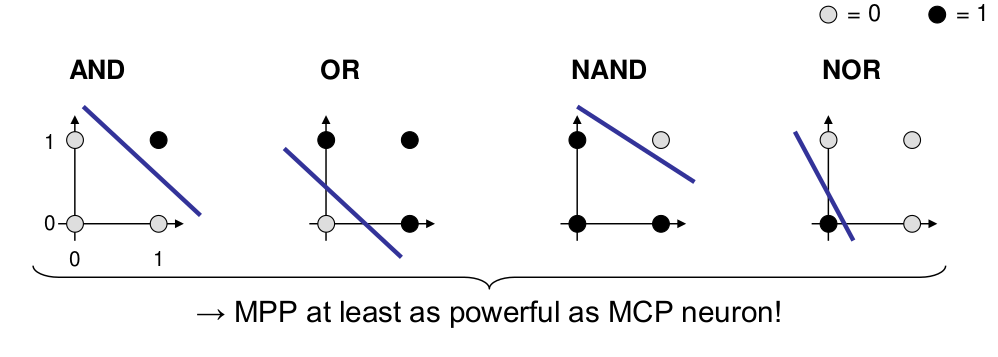
\includegraphics[width=1\textwidth]{MPP.png}
\\
To solve the xor functions a nonlinear function and an additional "neuron" is required.\\
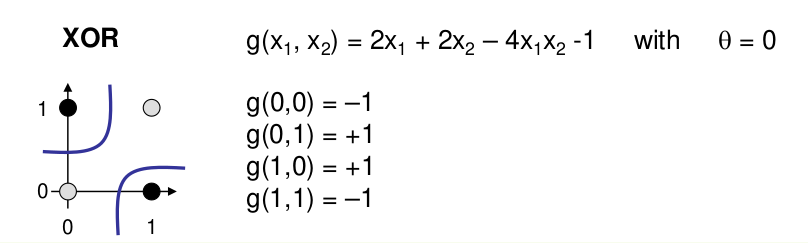
\includegraphics[width=1\textwidth]{XOR.png}
\\
So far all modules obtained their wheights and threshold by construction.\\
Now we want to have the neurons figure those out themselves, by training/ learning.\\
\subsection{Perceptron learning}
Let test examples with correct I/O - behaviour be given.\\
Following we apply the principle:
\begin{enumerate}
    \item choose initial weights in arbitrary number
    \item feed in test pattern
    \item if outpu of perceptron is wrong. then change the wheights
    \item goto (2.) until the output is correct for all test patterns
\end{enumerate}\ \\
We emerge the subsets $N$ and $P$ of the original dataset, with\\
$
N := \text{set of examples with negative output ($\forall x \in N. x = 0$)}\\
P := \text{set of examples with positive output ($\forall x \in P. x = 0$)}\\
$
\\
The algorithm Alg works by the following principle:
\begin{enumerate}
    \item choose $w_{t=0}$ randomly
    \item choose arbitrary $x \in P \cup N$
    \item   if $x \in P \land  w_t * x > 0$ then goto (2.) \\ 
            if $x \in N \land  w_t * x \leq 0$ then goto (2.)
    \item   if $x \in P \land w_t * x \leq 0$ then\\
            $w_{t+1} = w_t + x; ++t; goto(2.)$
    \item   if $x \in N \land w_t * x > 0$ then\\
            $w_{t+1} = w_t - x; ++t; goto(2.)$
    \item   (I/O correct for all examples) ? stop : run again
\end{enumerate}
A major drawback with this algorithm is:\\
$Alg \in O(exp)$
\subsubsection{What can multiple MPP do?}
As shown before a single MPP can seperate a plane in two halfes.\\
Therefore many MPP can in 2 layers can identify a convex set.\\
\end{document}
